\section{Discussion}
\label{sec:conclusions}

We have presented CHAODA (Clustered Hierarchical Anomaly and Outlier Detection Algorithms), a collection of five algorithms that exploit properties of a hierarchical cluster tree which represents an approximate manifold in $n$-dimensional space.
All five algorithms are trivial to implement on top of the manifold-learning framework we call CLAM (Clustered Learning of Approximate Manifolds); CHAODA builds on this framework similarly to CHESS~\cite{ishaq2019entropy}, which learns a manifold in the same way, but for the purpose of accelerating approximate search.
In CHESS, the geometric and topological properties of low fractal dimension and low metric entropy are advantages; indeed, CHESS does not perform particularly well if those properties are not present.
CHAODA, on the other hand, while competitive with other state-of-the-art anomaly-detection approaches on ``easy'' data sets (we define as \textit{easy} any data set where a one-class SVM performs well), outperforms other current methods when the data exhibit precisely those properties that CHESS depends on for acceleration. In particular, CHAODA outperforms other approaches on high-dimensional data sets, with the exception of the highest-dimensional dataset analyzed, ``annthyroid,'' where iForest and AOD perform better.

% note: make sure the above statement is actually true! Need to look at t-SNE and UMAP 
% for the breast cancer data set, as well as fractal dimension

\begin{figure}
    \centering
    % TODO!!
    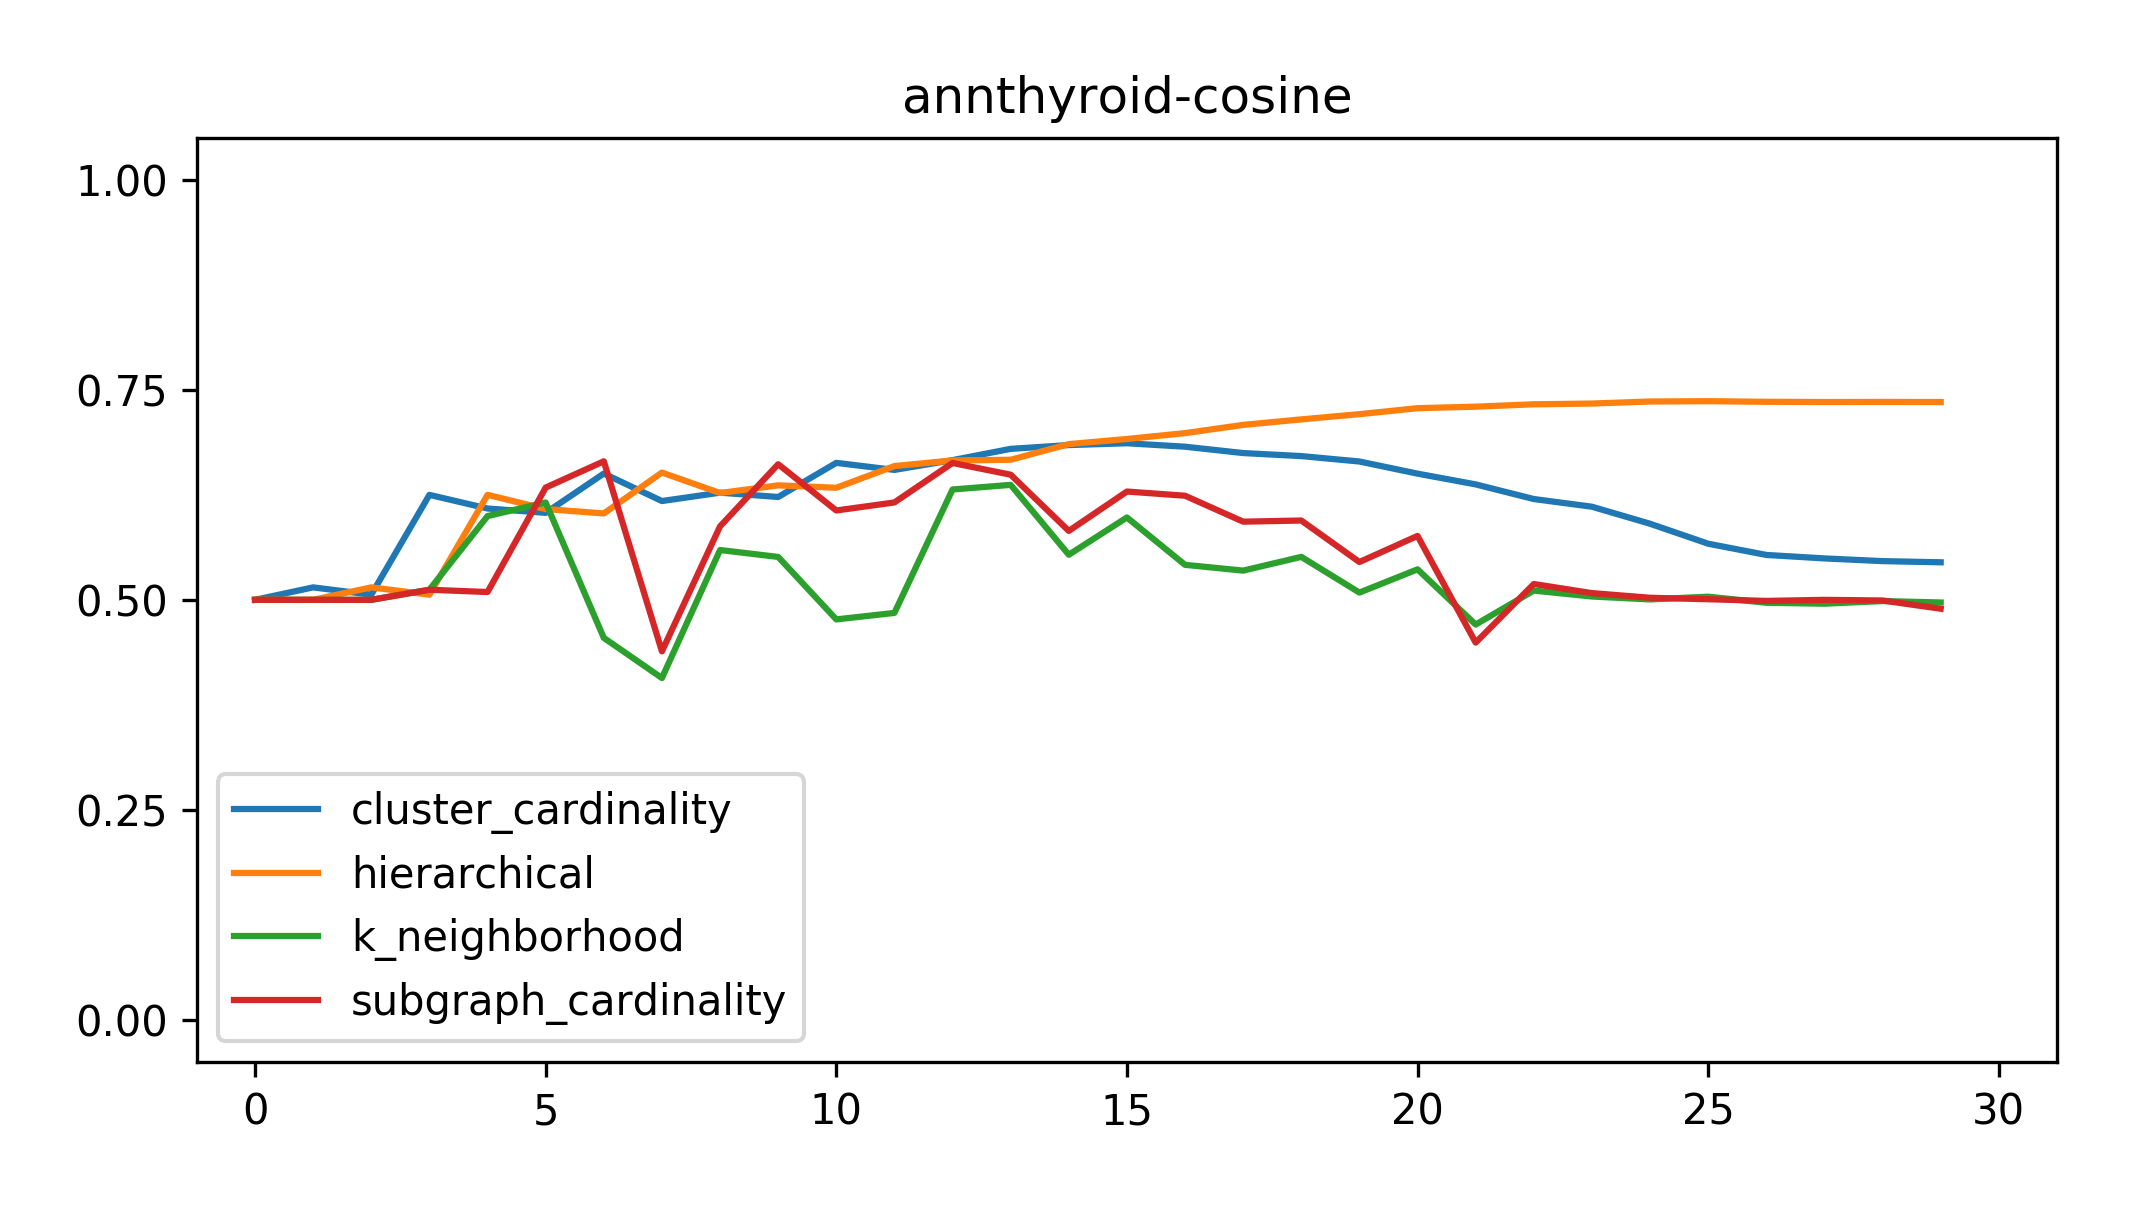
\includegraphics{kdd/static/auc_vs_depth/annthyroid-cosine.png}
    \caption{UMAP of Annthyroid Dataset}
    \label{fig:annthyroid-umap}
\end{figure}

With the sole exception of the annthyroid dataset, the algorithms presented here outperform or match all other approaches. 
At this point, it is important that we discuss some of the reasons that may be contributing to CHAODA's difficulty with this one dataset in particular.
Upon further investigation, it appears that this data may be in too few dimensions for CLAM to partition it into a useful manifold.
In UMAP projections we created on annthyroid~\ref{fig:annthyroid-umap}, it can be clearly seen that the anomalous data appears to live directly on the manifold, with only a small pocket appearing to be distinctly off.
This aligns perfectly with our expectations for CHAODA.
Indeed, the manifold being both learnable and distinctly separate from the anomalous data are mandatory properties for any of our approaches to be effective.
Fortunately, we can clearly see that these properties are apparent in all other datasets studied.

One current limitation in CHAODA is that the depth of the cluster tree at which anomaly detection performs best is not the same for every data set, and thus our results could be seen as ``cherry-picking'' from a scattershot approach.
This is because as depth increases, the induced graph ``shatters'', i.e. the number of components in the graph approaches the number of clusters in the graph.
Future work should certainly explore optimal stopping criteria so that we can automate stopping just before the graph shatters.
However, as shown in Figure~\ref{}, for most datasets, performance is not overly sensitive to the choice of depth.
We can treat depth as a hyperparameter to all of the methods described, but a detailed analysis of possible criteria for determining the optimal depth is essential future work.

% TODO: Need to look at local fractal dimension, or volume ratios, vs. optimal depth. Ideally we can say something like:
% The strong correlation between local fractal dimension and optimal tree depth suggests a guideline for determining an optimal tree depth directly from the data.

The choice of distance function also has a significant impact on anomaly-detection performance.
In this case, domain knowledge is likely the best way to determine the distance function of choice.
In future work, we seek to explore a more diverse collection of domain-appropriate distance functions, such as Wasserstein distance on images, and Levenshtein edit distance on strings. 

% TODO: Have we proved this?
% Say something about applying CHAODA for inputs to an ANN, in particular detecting just-off-manifold malicious inputs, like the school bus / ostrich example.

In conclusion, we have demonstrated that by learning approximate manifolds, we can exploit the embedded knowledge to implement trivial algorithms capable of outperforming other state-of-the-art approaches to anomaly detection.
